\documentclass{standalone}
\usepackage{graphicx}	
\usepackage{amssymb, amsmath, amsthm}
\usepackage{color}

\usepackage{tikz}
\usetikzlibrary{intersections, backgrounds}

\definecolor{light}{RGB}{220, 188, 188}
\definecolor{mid}{RGB}{185, 124, 124}
\definecolor{dark}{RGB}{143, 39, 39}
\definecolor{gray60}{gray}{0.6}
\definecolor{gray70}{gray}{0.7}
\definecolor{gray80}{gray}{0.8}
\definecolor{gray90}{gray}{0.90}
\definecolor{gray95}{gray}{0.95}

\newcommand{\mcpoint}[2]{  
  \fill[color=dark] (#1, #2) circle (7pt); 
  \fill[color=light] (#1, #2) circle (5pt);
}

\begin{document}

\begin{tikzpicture}[scale=0.25, thick]
  %\draw[blue] (-12, -9.5) rectangle (12, 6.5);

  \begin{scope}
    \clip (-12, -9.5) rectangle (12, 6.5);
 
    \foreach \i in {1, 0.99, ..., 0} {
      \pgfmathsetmacro{\prop}{100 * exp(-10.0 * \i * \i)};
      \colorlet{custom}{dark!\prop!white};
      \draw[line width={30 * \i}, color=custom] 
        (-5, 2) ellipse (5 and 3);
    }  
  
    \foreach \i in {1, 0.99, ..., 0} {
      \pgfmathsetmacro{\prop}{100 * exp(-10.0 * \i * \i)};
      \colorlet{custom}{dark!\prop!white};
      \draw[line width={30 * \i}, color=custom] 
        (5, -4.5) ellipse (5 and 3);
    }    
  \end{scope}
  
  \draw[<-, >=stealth, line width=0.5] (-11, -5) -- (-11, -8)
  node[right] {$\varpi_{v}(q)$};
    
  %\draw[blue] (16, -9.5) rectangle (40, 6.5);

  \node[] at (30,-2) {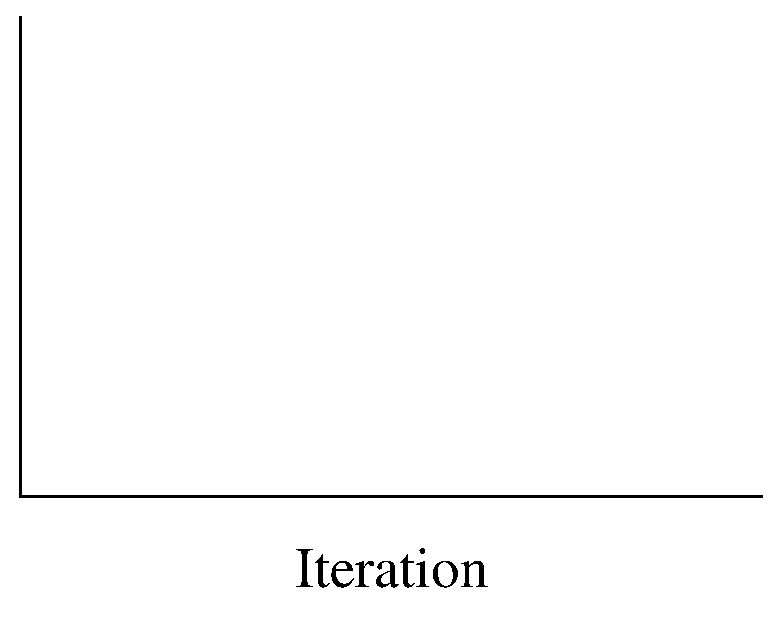
\includegraphics[width=5cm]{gnuplot/trace0.eps}};
  \node[rotate=90] at (18.5, -1) { $\varpi_{v}(q)$ };
  
  %\draw[blue] (44, -9.5) rectangle (68, 6.5);
  
  \node[] at (57,-2) {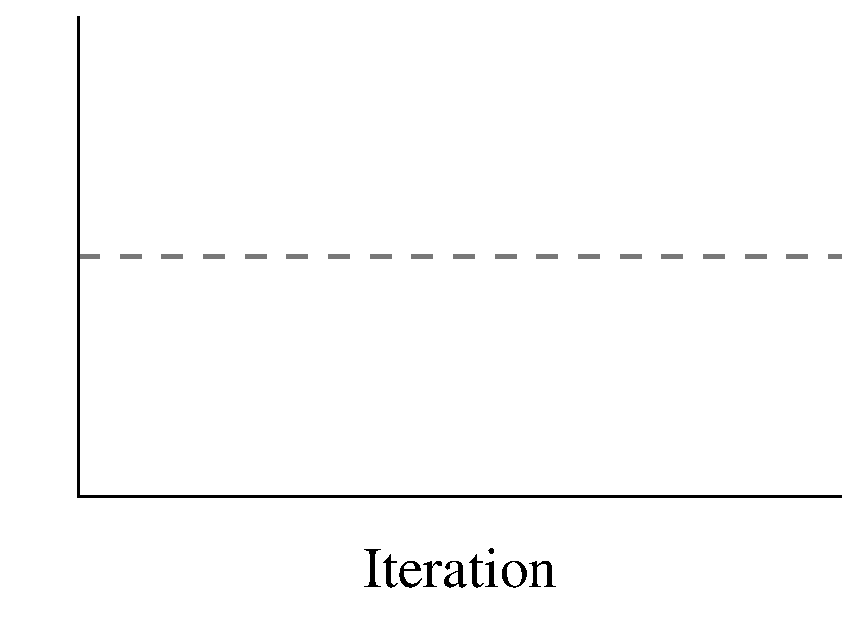
\includegraphics[width=5.5cm]{gnuplot/estimator_error_axes.eps}};
  \node[rotate=90] at (46, -0.75) { $\mathbb{E} \! \left[ \varpi_{v} \right] - \hat{\varpi}_{v}$ };
\end{tikzpicture}

\end{document}  